% Options for packages loaded elsewhere
\PassOptionsToPackage{unicode}{hyperref}
\PassOptionsToPackage{hyphens}{url}
%
\documentclass[
  8pt,
  ignorenonframetext,
]{beamer}
\usepackage{pgfpages}
\setbeamertemplate{caption}[numbered]
\setbeamertemplate{caption label separator}{: }
\setbeamercolor{caption name}{fg=normal text.fg}
\beamertemplatenavigationsymbolsempty
% Prevent slide breaks in the middle of a paragraph
\widowpenalties 1 10000
\raggedbottom
\setbeamertemplate{part page}{
  \centering
  \begin{beamercolorbox}[sep=16pt,center]{part title}
    \usebeamerfont{part title}\insertpart\par
  \end{beamercolorbox}
}
\setbeamertemplate{section page}{
  \centering
  \begin{beamercolorbox}[sep=12pt,center]{part title}
    \usebeamerfont{section title}\insertsection\par
  \end{beamercolorbox}
}
\setbeamertemplate{subsection page}{
  \centering
  \begin{beamercolorbox}[sep=8pt,center]{part title}
    \usebeamerfont{subsection title}\insertsubsection\par
  \end{beamercolorbox}
}
\AtBeginPart{
  \frame{\partpage}
}
\AtBeginSection{
  \ifbibliography
  \else
    \frame{\sectionpage}
  \fi
}
\AtBeginSubsection{
  \frame{\subsectionpage}
}
\usepackage{amsmath,amssymb}
\usepackage{lmodern}
\usepackage{iftex}
\ifPDFTeX
  \usepackage[T1]{fontenc}
  \usepackage[utf8]{inputenc}
  \usepackage{textcomp} % provide euro and other symbols
\else % if luatex or xetex
  \usepackage{unicode-math}
  \defaultfontfeatures{Scale=MatchLowercase}
  \defaultfontfeatures[\rmfamily]{Ligatures=TeX,Scale=1}
\fi
\usetheme[]{CambridgeUS}
% Use upquote if available, for straight quotes in verbatim environments
\IfFileExists{upquote.sty}{\usepackage{upquote}}{}
\IfFileExists{microtype.sty}{% use microtype if available
  \usepackage[]{microtype}
  \UseMicrotypeSet[protrusion]{basicmath} % disable protrusion for tt fonts
}{}
\makeatletter
\@ifundefined{KOMAClassName}{% if non-KOMA class
  \IfFileExists{parskip.sty}{%
    \usepackage{parskip}
  }{% else
    \setlength{\parindent}{0pt}
    \setlength{\parskip}{6pt plus 2pt minus 1pt}}
}{% if KOMA class
  \KOMAoptions{parskip=half}}
\makeatother
\usepackage{xcolor}
\newif\ifbibliography
\usepackage{color}
\usepackage{fancyvrb}
\newcommand{\VerbBar}{|}
\newcommand{\VERB}{\Verb[commandchars=\\\{\}]}
\DefineVerbatimEnvironment{Highlighting}{Verbatim}{commandchars=\\\{\}}
% Add ',fontsize=\small' for more characters per line
\usepackage{framed}
\definecolor{shadecolor}{RGB}{248,248,248}
\newenvironment{Shaded}{\begin{snugshade}}{\end{snugshade}}
\newcommand{\AlertTok}[1]{\textcolor[rgb]{0.94,0.16,0.16}{#1}}
\newcommand{\AnnotationTok}[1]{\textcolor[rgb]{0.56,0.35,0.01}{\textbf{\textit{#1}}}}
\newcommand{\AttributeTok}[1]{\textcolor[rgb]{0.77,0.63,0.00}{#1}}
\newcommand{\BaseNTok}[1]{\textcolor[rgb]{0.00,0.00,0.81}{#1}}
\newcommand{\BuiltInTok}[1]{#1}
\newcommand{\CharTok}[1]{\textcolor[rgb]{0.31,0.60,0.02}{#1}}
\newcommand{\CommentTok}[1]{\textcolor[rgb]{0.56,0.35,0.01}{\textit{#1}}}
\newcommand{\CommentVarTok}[1]{\textcolor[rgb]{0.56,0.35,0.01}{\textbf{\textit{#1}}}}
\newcommand{\ConstantTok}[1]{\textcolor[rgb]{0.00,0.00,0.00}{#1}}
\newcommand{\ControlFlowTok}[1]{\textcolor[rgb]{0.13,0.29,0.53}{\textbf{#1}}}
\newcommand{\DataTypeTok}[1]{\textcolor[rgb]{0.13,0.29,0.53}{#1}}
\newcommand{\DecValTok}[1]{\textcolor[rgb]{0.00,0.00,0.81}{#1}}
\newcommand{\DocumentationTok}[1]{\textcolor[rgb]{0.56,0.35,0.01}{\textbf{\textit{#1}}}}
\newcommand{\ErrorTok}[1]{\textcolor[rgb]{0.64,0.00,0.00}{\textbf{#1}}}
\newcommand{\ExtensionTok}[1]{#1}
\newcommand{\FloatTok}[1]{\textcolor[rgb]{0.00,0.00,0.81}{#1}}
\newcommand{\FunctionTok}[1]{\textcolor[rgb]{0.00,0.00,0.00}{#1}}
\newcommand{\ImportTok}[1]{#1}
\newcommand{\InformationTok}[1]{\textcolor[rgb]{0.56,0.35,0.01}{\textbf{\textit{#1}}}}
\newcommand{\KeywordTok}[1]{\textcolor[rgb]{0.13,0.29,0.53}{\textbf{#1}}}
\newcommand{\NormalTok}[1]{#1}
\newcommand{\OperatorTok}[1]{\textcolor[rgb]{0.81,0.36,0.00}{\textbf{#1}}}
\newcommand{\OtherTok}[1]{\textcolor[rgb]{0.56,0.35,0.01}{#1}}
\newcommand{\PreprocessorTok}[1]{\textcolor[rgb]{0.56,0.35,0.01}{\textit{#1}}}
\newcommand{\RegionMarkerTok}[1]{#1}
\newcommand{\SpecialCharTok}[1]{\textcolor[rgb]{0.00,0.00,0.00}{#1}}
\newcommand{\SpecialStringTok}[1]{\textcolor[rgb]{0.31,0.60,0.02}{#1}}
\newcommand{\StringTok}[1]{\textcolor[rgb]{0.31,0.60,0.02}{#1}}
\newcommand{\VariableTok}[1]{\textcolor[rgb]{0.00,0.00,0.00}{#1}}
\newcommand{\VerbatimStringTok}[1]{\textcolor[rgb]{0.31,0.60,0.02}{#1}}
\newcommand{\WarningTok}[1]{\textcolor[rgb]{0.56,0.35,0.01}{\textbf{\textit{#1}}}}
\usepackage{graphicx}
\makeatletter
\def\maxwidth{\ifdim\Gin@nat@width>\linewidth\linewidth\else\Gin@nat@width\fi}
\def\maxheight{\ifdim\Gin@nat@height>\textheight\textheight\else\Gin@nat@height\fi}
\makeatother
% Scale images if necessary, so that they will not overflow the page
% margins by default, and it is still possible to overwrite the defaults
% using explicit options in \includegraphics[width, height, ...]{}
\setkeys{Gin}{width=\maxwidth,height=\maxheight,keepaspectratio}
% Set default figure placement to htbp
\makeatletter
\def\fps@figure{htbp}
\makeatother
\setlength{\emergencystretch}{3em} % prevent overfull lines
\providecommand{\tightlist}{%
  \setlength{\itemsep}{0pt}\setlength{\parskip}{0pt}}
\setcounter{secnumdepth}{-\maxdimen} % remove section numbering
\ifLuaTeX
  \usepackage{selnolig}  % disable illegal ligatures
\fi
\IfFileExists{bookmark.sty}{\usepackage{bookmark}}{\usepackage{hyperref}}
\IfFileExists{xurl.sty}{\usepackage{xurl}}{} % add URL line breaks if available
\urlstyle{same} % disable monospaced font for URLs
\hypersetup{
  pdftitle={Intro to programming 2},
  hidelinks,
  pdfcreator={LaTeX via pandoc}}

\title{Intro to programming 2}
\author{Henri Vandendriessche\\
\href{mailto:henri.vandendriessche@ens.fr}{\nolinkurl{henri.vandendriessche@ens.fr}}}
\date{2022-09-27}

\begin{document}
\frame{\titlepage}

\begin{frame}[fragile]{Terminal cheat sheet reminder}
\protect\hypertarget{terminal-cheat-sheet-reminder}{}
\begin{itemize}
\item
  Bash commands to navigate directories

  \begin{itemize}
  \tightlist
  \item
    Print Working Directory. Print the path of the current directory
  \end{itemize}

\begin{Shaded}
\begin{Highlighting}[]
\BuiltInTok{pwd}
\end{Highlighting}
\end{Shaded}

  \begin{itemize}
  \tightlist
  \item
    List all files of the current directory
  \end{itemize}

\begin{Shaded}
\begin{Highlighting}[]
\FunctionTok{ls}\NormalTok{ folder}
\end{Highlighting}
\end{Shaded}

  \begin{itemize}
  \tightlist
  \item
    Moving into folder1 and subfolder2 at once.
  \end{itemize}

\begin{Shaded}
\begin{Highlighting}[]
\BuiltInTok{cd}\NormalTok{ folder1/subfolder2}
\end{Highlighting}
\end{Shaded}

  \begin{itemize}
  \tightlist
  \item
    Moving out of a directory
  \end{itemize}

\begin{Shaded}
\begin{Highlighting}[]
\BuiltInTok{cd}\NormalTok{ ..}
\end{Highlighting}
\end{Shaded}

  \begin{itemize}
  \tightlist
  \item
    Going back to the root directory
  \end{itemize}

\begin{Shaded}
\begin{Highlighting}[]
\BuiltInTok{cd}\NormalTok{ \textasciitilde{}}
\end{Highlighting}
\end{Shaded}
\item
  ``\textbf{Tab}'' to use the auto-completion
\item
  \textbf{Ctrl + C} to stop a program execution
\item
  Many more bash commands to use\ldots{}
\end{itemize}
\end{frame}

\begin{frame}{So far}
\protect\hypertarget{so-far}{}
\begin{itemize}
\item
  Python
\item
  Variables
\item
  Data types:

  \begin{itemize}
  \tightlist
  \item
    integer
  \item
    float
  \item
    string
  \item
    boolean
  \end{itemize}
\item
  If and For loops:

  \begin{itemize}
  \tightlist
  \item
    syntax use the right keywords \textbf{if}, \textbf{elif},
    \textbf{else}, \textbf{for}, \textbf{in} and don't forget the
    \textbf{:}
  \item
    indentation
  \end{itemize}
\end{itemize}
\end{frame}

\begin{frame}{Reading advice}
\protect\hypertarget{reading-advice}{}
To complete what we're going to see today.

\begin{itemize}
\item
  \url{https://automatetheboringstuff.com/2e/chapter4/}
\item
  \url{https://automatetheboringstuff.com/2e/chapter5/}
\end{itemize}
\end{frame}

\begin{frame}{Today}
\protect\hypertarget{today}{}
\begin{itemize}
\item
  Constant and Variable
\item
  While loop
\item
  Other python data types for collections of data type

  \begin{itemize}
  \item
    list
  \item
    set
  \item
    tuple
  \item
    dictionary
  \end{itemize}
\item
  Exercises
\end{itemize}
\end{frame}

\begin{frame}[fragile]{Constant vs Variable}
\protect\hypertarget{constant-vs-variable}{}
\begin{itemize}[<+->]
\tightlist
\item
  So far we have seen how to declare, instantiate and modify variables
\end{itemize}

\begin{itemize}[<+->]
\tightlist
\item
  But there are ``variables'' that you don't want to modify and
  traditionally in programming those variables are called constant
\end{itemize}

\begin{itemize}[<+->]
\item
  Unfortunately there is no native way of declaring a constant in
  python. However there is a unwritten convention that you use only
  upper case

\begin{Shaded}
\begin{Highlighting}[]
\NormalTok{CONST\_PI }\OperatorTok{=} \FloatTok{3.1415}
\end{Highlighting}
\end{Shaded}
\end{itemize}

\begin{itemize}[<+->]
\item
  Python include in its core library some constants

\begin{Shaded}
\begin{Highlighting}[]
\ImportTok{import}\NormalTok{ math}

\NormalTok{math.pi}
\end{Highlighting}
\end{Shaded}

\begin{verbatim}
## 3.141592653589793
\end{verbatim}
\end{itemize}
\end{frame}

\begin{frame}{While loop 1/3}
\protect\hypertarget{while-loop-13}{}
\begin{itemize}[<+->]
\tightlist
\item
  \textbf{While} loop will keep looping all over again an ending
  instruction is met.
\end{itemize}

\begin{itemize}[<+->]
\tightlist
\item
  As the \textbf{for} loop incorporate a specified number of execution,
  the \textbf{while} loop is best suited for unknown or very large
  number of loop iterations.
\end{itemize}

\begin{itemize}[<+->]
\tightlist
\item
  As for \textbf{if} and \textbf{for}, \textbf{while} has a syntax with
  `\textbf{:}' and need indentation for the following lines to be
  included in the process
\end{itemize}

\begin{itemize}[<+->]
\tightlist
\item
  The two key features of a while loop are:

  \begin{itemize}[<+->]
  \tightlist
  \item
    the output condition
  \item
    the increment statement
  \end{itemize}
\end{itemize}
\end{frame}

\begin{frame}[fragile]{While loop 2/3}
\protect\hypertarget{while-loop-23}{}
\begin{itemize}[<+->]
\tightlist
\item
  Example :
\end{itemize}

\begin{quote}
\begin{Shaded}
\begin{Highlighting}[]
\NormalTok{i }\OperatorTok{=} \DecValTok{1}
\ControlFlowTok{while}\NormalTok{ i }\OperatorTok{\textless{}} \DecValTok{4}\NormalTok{: }\CommentTok{\#  output condition}
  \BuiltInTok{print}\NormalTok{(i)}
\NormalTok{  i }\OperatorTok{+=} \DecValTok{1}     \CommentTok{\# increment statement}
\end{Highlighting}
\end{Shaded}

\begin{verbatim}
## 1
## 2
## 3
\end{verbatim}
\end{quote}

\begin{itemize}[<+->]
\item
  Which is technically the same as

\begin{Shaded}
\begin{Highlighting}[]
\ControlFlowTok{for}\NormalTok{ i }\KeywordTok{in} \BuiltInTok{range}\NormalTok{(}\DecValTok{1}\NormalTok{,}\DecValTok{4}\NormalTok{):}
  \BuiltInTok{print}\NormalTok{(i)}
\end{Highlighting}
\end{Shaded}

\begin{verbatim}
## 1
## 2
## 3
\end{verbatim}
\end{itemize}
\end{frame}

\begin{frame}[fragile]{While loop 3/3}
\protect\hypertarget{while-loop-33}{}
\begin{itemize}[<+->]
\tightlist
\item
  \textbf{While} loop will test if the output condition is True and if
  not it will execute the code and execute the increment statement
\end{itemize}

\begin{itemize}[<+->]
\item
  If one of those two conditions are not correctly specified you'll
  encounter an error or an infinite loop\ldots{}
\item
  Example 1

\begin{Shaded}
\begin{Highlighting}[]
\NormalTok{i }\OperatorTok{=} \DecValTok{1}
\ControlFlowTok{while}\NormalTok{ i }\OperatorTok{\textless{}} \DecValTok{6}\NormalTok{: }\CommentTok{\#  output condition}
  \BuiltInTok{print}\NormalTok{(i)}
\end{Highlighting}
\end{Shaded}
\end{itemize}

\begin{itemize}[<+->]
\item
  Example 2

\begin{Shaded}
\begin{Highlighting}[]
\NormalTok{i }\OperatorTok{=} \DecValTok{1}
\ControlFlowTok{while}\NormalTok{ i }\OperatorTok{!=} \DecValTok{6}\NormalTok{:}
  \BuiltInTok{print}\NormalTok{(i)}
\NormalTok{  i }\OperatorTok{+=} \DecValTok{2}
\end{Highlighting}
\end{Shaded}
\end{itemize}
\end{frame}

\begin{frame}[fragile]{Breaking a loop 1/2}
\protect\hypertarget{breaking-a-loop-12}{}
\begin{itemize}
\tightlist
\item
  Breaking a loop is possible using \textbf{break}. For example when the
  rest of a loop is useless
\end{itemize}

\begin{Shaded}
\begin{Highlighting}[]
\CommentTok{\# Checking if a number is primitive}
\NormalTok{N }\OperatorTok{=} \DecValTok{72239}
\ControlFlowTok{for}\NormalTok{ i }\KeywordTok{in} \BuiltInTok{range}\NormalTok{(}\DecValTok{2}\NormalTok{, }\DecValTok{300}\NormalTok{):}
  \ControlFlowTok{if}\NormalTok{ N }\OperatorTok{\%}\NormalTok{ i }\OperatorTok{==} \DecValTok{0}\NormalTok{:}
    \BuiltInTok{print}\NormalTok{(i)}
    \ControlFlowTok{break} 
\end{Highlighting}
\end{Shaded}

\begin{verbatim}
## 29
\end{verbatim}

\begin{itemize}
\tightlist
\item
  Other example
\end{itemize}

\begin{Shaded}
\begin{Highlighting}[]
\CommentTok{\# Checking a password}
\NormalTok{passwd }\OperatorTok{=} \StringTok{\textquotesingle{}sesame\textquotesingle{}}

\ControlFlowTok{while} \VariableTok{True}\NormalTok{:}
\NormalTok{  code }\OperatorTok{=} \BuiltInTok{input}\NormalTok{(}\StringTok{\textquotesingle{}Password? \textquotesingle{}}\NormalTok{)}
  \ControlFlowTok{if}\NormalTok{ code }\OperatorTok{==}\NormalTok{ passwd:}
    \ControlFlowTok{break}
  \ControlFlowTok{else}\NormalTok{:}
    \BuiltInTok{print}\NormalTok{(}\StringTok{\textquotesingle{}invalid password\textquotesingle{}}\NormalTok{)}

\BuiltInTok{print}\NormalTok{(}\StringTok{"You are in!"}\NormalTok{)}
\end{Highlighting}
\end{Shaded}
\end{frame}

\begin{frame}[fragile]{Breaking a loop 2/2}
\protect\hypertarget{breaking-a-loop-22}{}
\begin{itemize}
\tightlist
\item
  The keyword \textbf{continue} is also very useful to pass the current
  iteration
\end{itemize}

\begin{Shaded}
\begin{Highlighting}[]
\ControlFlowTok{for}\NormalTok{ i }\KeywordTok{in} \BuiltInTok{range}\NormalTok{(}\DecValTok{0}\NormalTok{,}\DecValTok{5}\NormalTok{):}
  \ControlFlowTok{if}\NormalTok{ i }\OperatorTok{==} \DecValTok{3}\NormalTok{:}
    \ControlFlowTok{continue}
  \ControlFlowTok{else}\NormalTok{:}
    \BuiltInTok{print}\NormalTok{(i)}
\end{Highlighting}
\end{Shaded}

\begin{verbatim}
## 0
## 1
## 2
## 4
\end{verbatim}
\end{frame}

\begin{frame}[fragile]{Lists 1/3}
\protect\hypertarget{lists-13}{}
\begin{itemize}[<+->]
\tightlist
\item
  A list is a collection of related objects
\end{itemize}

\begin{itemize}[<+->]
\tightlist
\item
  It's declared with brackets {[}{]} with a comma between two objects
\end{itemize}

\begin{itemize}[<+->]
\item
  Example 1

\begin{Shaded}
\begin{Highlighting}[]
\NormalTok{Years\_France\_won\_worldcup }\OperatorTok{=}\NormalTok{ [}\DecValTok{1998}\NormalTok{, }\DecValTok{2018}\NormalTok{]}
\BuiltInTok{print}\NormalTok{(Years\_France\_won\_worldcup)}
\end{Highlighting}
\end{Shaded}

\begin{verbatim}
## [1998, 2018]
\end{verbatim}
\end{itemize}

\begin{itemize}[<+->]
\item
  Example 2

\begin{Shaded}
\begin{Highlighting}[]
\NormalTok{dog\_breeds }\OperatorTok{=}\NormalTok{ [}\StringTok{"golden"}\NormalTok{, }\StringTok{"corgi"}\NormalTok{, }\StringTok{"Bulldog"}\NormalTok{, }\StringTok{"Husky"}\NormalTok{, }\StringTok{"Beagle"}\NormalTok{]}
\NormalTok{dog\_breeds2 }\OperatorTok{=}\NormalTok{ [}\StringTok{"golden"} \StringTok{"corgi"} \StringTok{"Bulldog"} \StringTok{"Husky"} \StringTok{"Beagle"}\NormalTok{]}
\BuiltInTok{print}\NormalTok{(dog\_breeds)}
\end{Highlighting}
\end{Shaded}

\begin{verbatim}
## ['golden', 'corgi', 'Bulldog', 'Husky', 'Beagle']
\end{verbatim}

\begin{Shaded}
\begin{Highlighting}[]
\BuiltInTok{print}\NormalTok{(dog\_breeds2)}
\end{Highlighting}
\end{Shaded}

\begin{verbatim}
## ['goldencorgiBulldogHuskyBeagle']
\end{verbatim}
\end{itemize}

\begin{itemize}[<+->]
\item
  Example 3

\begin{Shaded}
\begin{Highlighting}[]
\NormalTok{random\_data\_type\_collection }\OperatorTok{=}\NormalTok{ [ }\DecValTok{1}\NormalTok{, }\VariableTok{True}\NormalTok{, }\StringTok{"Cats"}\NormalTok{, }\FloatTok{3.14}\NormalTok{]}
\BuiltInTok{print}\NormalTok{(random\_data\_type\_collection)}
\end{Highlighting}
\end{Shaded}

\begin{verbatim}
## [1, True, 'Cats', 3.14]
\end{verbatim}
\end{itemize}
\end{frame}

\begin{frame}[fragile]{Lists 2/3}
\protect\hypertarget{lists-23}{}
\begin{itemize}
\tightlist
\item
  Access element in a list through its index which is the same to access
  characters in a string as in a list
\end{itemize}

\begin{Shaded}
\begin{Highlighting}[]
\NormalTok{prog\_language }\OperatorTok{=}\NormalTok{ [}\StringTok{"python"}\NormalTok{, }\StringTok{"R"}\NormalTok{, }\StringTok{"C"}\NormalTok{, }\StringTok{"java"}\NormalTok{, }\StringTok{"Go"}\NormalTok{, }\StringTok{"Rust"}\NormalTok{]}
\BuiltInTok{print}\NormalTok{(prog\_language[}\DecValTok{0}\NormalTok{])}
\end{Highlighting}
\end{Shaded}

\begin{verbatim}
## python
\end{verbatim}

\begin{Shaded}
\begin{Highlighting}[]
\BuiltInTok{print}\NormalTok{(prog\_language[}\OperatorTok{{-}}\DecValTok{1}\NormalTok{])}
\end{Highlighting}
\end{Shaded}

\begin{verbatim}
## Rust
\end{verbatim}

\begin{Shaded}
\begin{Highlighting}[]
\NormalTok{programming\_language }\OperatorTok{=} \StringTok{"python"}
\BuiltInTok{print}\NormalTok{(programming\_language[}\DecValTok{0}\NormalTok{])}
\end{Highlighting}
\end{Shaded}

\begin{verbatim}
## p
\end{verbatim}

\begin{Shaded}
\begin{Highlighting}[]
\BuiltInTok{print}\NormalTok{(}\BuiltInTok{type}\NormalTok{(programming\_language))}
\end{Highlighting}
\end{Shaded}

\begin{verbatim}
## <class 'str'>
\end{verbatim}
\end{frame}

\begin{frame}[fragile]{Lists 3/3}
\protect\hypertarget{lists-33}{}
\begin{itemize}[<+->]
\tightlist
\item
  As for the any other variables lists can be used with functions

  \begin{itemize}[<+->]
  \tightlist
  \item
    append()
  \item
    remove()
  \item
    pop()
  \item
    sort()
  \item
    len()
  \end{itemize}
\end{itemize}

\begin{itemize}[<+->]
\item
  Example

\begin{Shaded}
\begin{Highlighting}[]
\NormalTok{prog\_language }\OperatorTok{=}\NormalTok{ [}\StringTok{"python"}\NormalTok{, }\StringTok{"R"}\NormalTok{, }\StringTok{"C"}\NormalTok{, }\StringTok{"java"}\NormalTok{, }\StringTok{"Go"}\NormalTok{, }\StringTok{"Rust"}\NormalTok{]}
\NormalTok{prog\_language.append(}\StringTok{"html"}\NormalTok{)}
\NormalTok{prog\_language.append(}\StringTok{"PHP"}\NormalTok{)}
\BuiltInTok{print}\NormalTok{(prog\_language)}
\end{Highlighting}
\end{Shaded}

\begin{verbatim}
## ['python', 'R', 'C', 'java', 'Go', 'Rust', 'html', 'PHP']
\end{verbatim}

\begin{Shaded}
\begin{Highlighting}[]
\NormalTok{prog\_language.remove(}\StringTok{"html"}\NormalTok{)}

\BuiltInTok{len}\NormalTok{(prog\_language)}
\end{Highlighting}
\end{Shaded}

\begin{verbatim}
## 7
\end{verbatim}

\begin{Shaded}
\begin{Highlighting}[]
\NormalTok{prog\_language.sort()}
\BuiltInTok{print}\NormalTok{(prog\_language)}
\end{Highlighting}
\end{Shaded}

\begin{verbatim}
## ['C', 'Go', 'PHP', 'R', 'Rust', 'java', 'python']
\end{verbatim}
\end{itemize}
\end{frame}

\begin{frame}[fragile]{Tuples 1/3}
\protect\hypertarget{tuples-13}{}
\begin{itemize}[<+->]
\tightlist
\item
  Very similar to Lists and is used for data collection
\end{itemize}

\begin{itemize}[<+->]
\tightlist
\item
  Declared with ``\textbf{()}'' instead of square bracket and with a
  ``\textbf{,}''
\end{itemize}

\begin{itemize}[<+->]
\item
  Example

\begin{Shaded}
\begin{Highlighting}[]
\NormalTok{date\_covid\_shots }\OperatorTok{=}\NormalTok{ (}\StringTok{"21{-}04{-}15"}\NormalTok{, }\StringTok{"21{-}05{-}18"}\NormalTok{, }\StringTok{"21{-}09{-}20"}\NormalTok{)}

\BuiltInTok{print}\NormalTok{(}\BuiltInTok{type}\NormalTok{(date\_covid\_shots))}
\end{Highlighting}
\end{Shaded}

\begin{verbatim}
## <class 'tuple'>
\end{verbatim}

\begin{Shaded}
\begin{Highlighting}[]
\BuiltInTok{print}\NormalTok{(date\_covid\_shots[}\DecValTok{1}\NormalTok{])  }\CommentTok{\# Accessible as list with index with []}
\end{Highlighting}
\end{Shaded}

\begin{verbatim}
## 21-05-18
\end{verbatim}

\begin{Shaded}
\begin{Highlighting}[]
\BuiltInTok{print}\NormalTok{(}\BuiltInTok{len}\NormalTok{(date\_covid\_shots))}
\end{Highlighting}
\end{Shaded}

\begin{verbatim}
## 3
\end{verbatim}
\end{itemize}
\end{frame}

\begin{frame}[fragile]{Tuples 2/3}
\protect\hypertarget{tuples-23}{}
\begin{itemize}[<+->]
\item
  In contrast to lists, they are immutable and can't be modified.

\begin{Shaded}
\begin{Highlighting}[]
\NormalTok{date\_covid\_shots }\OperatorTok{=}\NormalTok{ (}\StringTok{"21{-}04{-}15"}\NormalTok{, }\StringTok{"21{-}05{-}18"}\NormalTok{, }\StringTok{"21{-}09{-}20"}\NormalTok{)}
\NormalTok{date\_covid\_shots.append(}\StringTok{"21{-}09{-}27"}\NormalTok{)}
\end{Highlighting}
\end{Shaded}

\begin{verbatim}
## Error in py_call_impl(callable, dots$args, dots$keywords): AttributeError: 'tuple' object has no attribute 'append'
\end{verbatim}
\end{itemize}

\begin{itemize}[<+->]
\tightlist
\item
  You can't change the order of items neither modify the value of an
  item
\end{itemize}

\begin{itemize}[<+->]
\tightlist
\item
  Tuples are best suited when you need ordered lists that would never
  change

  \begin{itemize}[<+->]
  \tightlist
  \item
    If you want to code a calendar : days and years can be coded as
    tuples as they would not change but are ordered.
  \end{itemize}
\end{itemize}
\end{frame}

\begin{frame}[fragile]{Tuples 3/3}
\protect\hypertarget{tuples-33}{}
\begin{itemize}[<+->]
\item
  Note that you could combine lists and tuples

\begin{Shaded}
\begin{Highlighting}[]
\NormalTok{Cocktails }\OperatorTok{=}\NormalTok{ [(}\StringTok{"Cosmo"}\NormalTok{,}\StringTok{"5€"}\NormalTok{),(}\StringTok{"Daiquiri"}\NormalTok{,}\StringTok{"7€"}\NormalTok{),(}\StringTok{"B52"}\NormalTok{,}\StringTok{"6€"}\NormalTok{)]}
\NormalTok{Cocktails.append((}\StringTok{"Mojito"}\NormalTok{,}\StringTok{"7€"}\NormalTok{))}

\BuiltInTok{print}\NormalTok{(Cocktails)}
\end{Highlighting}
\end{Shaded}

\begin{verbatim}
## [('Cosmo', '5€'), ('Daiquiri', '7€'), ('B52', '6€'), ('Mojito', '7€')]
\end{verbatim}
\end{itemize}

\begin{itemize}[<+->]
\item
  NB: you can also declare a tuple using a tuple() constructor

\begin{Shaded}
\begin{Highlighting}[]
\NormalTok{date\_covid\_shots }\OperatorTok{=} \BuiltInTok{tuple}\NormalTok{([}\StringTok{"21{-}04{-}15"}\NormalTok{, }\StringTok{"21{-}05{-}18"}\NormalTok{, }\StringTok{"21{-}09{-}20"}\NormalTok{])}
\CommentTok{\# in this line you transform a list into a tuple}
\BuiltInTok{print}\NormalTok{(}\BuiltInTok{type}\NormalTok{(date\_covid\_shots))}
\end{Highlighting}
\end{Shaded}

\begin{verbatim}
## <class 'tuple'>
\end{verbatim}
\end{itemize}
\end{frame}

\begin{frame}[fragile]{Sets 1/2}
\protect\hypertarget{sets-12}{}
\begin{itemize}[<+->]
\tightlist
\item
  Very close to lists but are unordered unindexed and do not allow
  duplicate value BUT are mutable
\end{itemize}

\begin{itemize}[<+->]
\tightlist
\item
  Declared with \{\}
\end{itemize}

\begin{itemize}[<+->]
\item
  Example

\begin{Shaded}
\begin{Highlighting}[]
\NormalTok{fruit\_I\_like }\OperatorTok{=}\NormalTok{ \{}\StringTok{"apple"}\NormalTok{, }\StringTok{"pineapple"}\NormalTok{, }\StringTok{"peach"}\NormalTok{\}}
\BuiltInTok{print}\NormalTok{(}\BuiltInTok{type}\NormalTok{(fruit\_I\_like))}
\end{Highlighting}
\end{Shaded}

\begin{verbatim}
## <class 'set'>
\end{verbatim}

\begin{Shaded}
\begin{Highlighting}[]
\BuiltInTok{print}\NormalTok{(fruit\_I\_like)}
\end{Highlighting}
\end{Shaded}

\begin{verbatim}
## {'apple', 'pineapple', 'peach'}
\end{verbatim}

\begin{Shaded}
\begin{Highlighting}[]
\NormalTok{fruit\_I\_like.add(}\StringTok{"strawberry"}\NormalTok{)}
\CommentTok{"strawberry"} \KeywordTok{in}\NormalTok{ fruit\_I\_like }\CommentTok{\# Check if a fruit is in my set}
\end{Highlighting}
\end{Shaded}

\begin{verbatim}
## True
\end{verbatim}

\begin{Shaded}
\begin{Highlighting}[]
\NormalTok{fruit\_I\_like.remove(}\StringTok{"apple"}\NormalTok{)}
\BuiltInTok{print}\NormalTok{(fruit\_I\_like)}
\end{Highlighting}
\end{Shaded}

\begin{verbatim}
## {'strawberry', 'pineapple', 'peach'}
\end{verbatim}
\end{itemize}
\end{frame}

\begin{frame}[fragile]{Sets 2/2}
\protect\hypertarget{sets-22}{}
\begin{itemize}[<+->]
\item
  But can't add/remove items in a set or access to item with index.
  Following instructions should throw an error

\begin{Shaded}
\begin{Highlighting}[]
\NormalTok{fruit\_I\_like[}\DecValTok{0}\NormalTok{]}
\end{Highlighting}
\end{Shaded}

\begin{verbatim}
## Error in py_call_impl(callable, dots$args, dots$keywords): TypeError: 'set' object is not subscriptable
\end{verbatim}

\begin{Shaded}
\begin{Highlighting}[]
\NormalTok{fruit\_I\_like.append(}\StringTok{"banana"}\NormalTok{)}
\end{Highlighting}
\end{Shaded}

\begin{verbatim}
## Error in py_call_impl(callable, dots$args, dots$keywords): AttributeError: 'set' object has no attribute 'append'
\end{verbatim}
\end{itemize}

\begin{itemize}
\tightlist
\item
  append() doesn't work cause it imply an order to add an item at the
  end
\end{itemize}

\begin{itemize}[<+->]
\item
  NB: you can also declare a set using a set() constructor (as for the
  tuple)

\begin{Shaded}
\begin{Highlighting}[]
\NormalTok{date\_covid\_shots }\OperatorTok{=} \BuiltInTok{set}\NormalTok{([}\StringTok{"21{-}04{-}15"}\NormalTok{, }\StringTok{"21{-}05{-}18"}\NormalTok{, }\StringTok{"21{-}09{-}20"}\NormalTok{])}
\CommentTok{\# in this line you transform a list into a tuple}
\BuiltInTok{print}\NormalTok{(}\BuiltInTok{type}\NormalTok{(date\_covid\_shots))}
\end{Highlighting}
\end{Shaded}

\begin{verbatim}
## <class 'set'>
\end{verbatim}
\end{itemize}
\end{frame}

\begin{frame}{Dictionaries 1/5}
\protect\hypertarget{dictionaries-15}{}
\begin{itemize}[<+->]
\tightlist
\item
  Data structure that uses data in key-value pairs.
\end{itemize}

\begin{itemize}[<+->]
\tightlist
\item
  Each items of a dictionary is a key-value pair
\end{itemize}

\begin{itemize}[<+->]
\tightlist
\item
  Each key has to be unique
\end{itemize}

\begin{itemize}[<+->]
\tightlist
\item
  Declared in a very specific way

  \begin{itemize}[<+->]
  \tightlist
  \item
    my\_dictionary = \{ ``key1'' : value1, ``key2'': value2 \ldots\}
  \end{itemize}
\end{itemize}
\end{frame}

\begin{frame}[fragile]{Dictionaries 2/5}
\protect\hypertarget{dictionaries-25}{}
\begin{itemize}[<+->]
\item
  Example

\begin{Shaded}
\begin{Highlighting}[]
\NormalTok{PCBS }\OperatorTok{=}\NormalTok{ \{}
\StringTok{"Name"}\NormalTok{ : }\StringTok{"PCBS"}\NormalTok{,}
\StringTok{"Teacher"}\NormalTok{ : }\StringTok{"Christophe Pallier"}\NormalTok{,}
\StringTok{"Teacher assistant"}\NormalTok{ : }\StringTok{"Henri"}\NormalTok{,}
\StringTok{"Course"}\NormalTok{ : [}\StringTok{"1"}\NormalTok{, }\StringTok{"2"}\NormalTok{],}
\StringTok{"Day"}\NormalTok{: }\StringTok{"Tuesday"}\NormalTok{,}
\StringTok{"Duration"}\NormalTok{ : }\DecValTok{3}\NormalTok{,}
\StringTok{"Mandatory"}\NormalTok{ : }\VariableTok{False}\NormalTok{\}}

\BuiltInTok{print}\NormalTok{(PCBS[}\StringTok{"Name"}\NormalTok{])}
\end{Highlighting}
\end{Shaded}

\begin{verbatim}
## PCBS
\end{verbatim}

\begin{Shaded}
\begin{Highlighting}[]
\BuiltInTok{print}\NormalTok{(PCBS[}\StringTok{"Teacher"}\NormalTok{])}
\end{Highlighting}
\end{Shaded}

\begin{verbatim}
## Christophe Pallier
\end{verbatim}

\begin{Shaded}
\begin{Highlighting}[]
\BuiltInTok{print}\NormalTok{(PCBS[}\StringTok{"Teacher assistant"}\NormalTok{])}
\end{Highlighting}
\end{Shaded}

\begin{verbatim}
## Henri
\end{verbatim}

\begin{Shaded}
\begin{Highlighting}[]
\BuiltInTok{print}\NormalTok{(PCBS[}\StringTok{"Course"}\NormalTok{])}
\end{Highlighting}
\end{Shaded}

\begin{verbatim}
## ['1', '2']
\end{verbatim}

\begin{Shaded}
\begin{Highlighting}[]
\BuiltInTok{print}\NormalTok{(PCBS[}\StringTok{"Day"}\NormalTok{])}
\end{Highlighting}
\end{Shaded}

\begin{verbatim}
## Tuesday
\end{verbatim}

\begin{Shaded}
\begin{Highlighting}[]
\BuiltInTok{print}\NormalTok{(PCBS[}\StringTok{"Duration"}\NormalTok{])}
\end{Highlighting}
\end{Shaded}

\begin{verbatim}
## 3
\end{verbatim}

\begin{Shaded}
\begin{Highlighting}[]
\BuiltInTok{print}\NormalTok{(PCBS[}\StringTok{"Mandatory"}\NormalTok{])}
\end{Highlighting}
\end{Shaded}

\begin{verbatim}
## False
\end{verbatim}
\end{itemize}
\end{frame}

\begin{frame}[fragile]{Dictionaries 3/5 Create a Dictionary}
\protect\hypertarget{dictionaries-35-create-a-dictionary}{}
\begin{itemize}[<+->]
\tightlist
\item
  You have several methods to create a dictionary:
\end{itemize}

\begin{itemize}[<+->]
\item
  Example1

\begin{Shaded}
\begin{Highlighting}[]
\NormalTok{PCBS }\OperatorTok{=}\NormalTok{ \{\}}
\NormalTok{PCBS[}\StringTok{"Name"}\NormalTok{] }\OperatorTok{=} \StringTok{"PCBS"}
\NormalTok{PCBS[}\StringTok{"Teacher"}\NormalTok{] }\OperatorTok{=} \StringTok{"Christophe Pallier"}
\NormalTok{PCBS[}\StringTok{"Teacher assistant"}\NormalTok{] }\OperatorTok{=} \StringTok{"Henri"}
\NormalTok{PCBS[}\StringTok{"Course"}\NormalTok{] }\OperatorTok{=}\NormalTok{ [}\StringTok{"1"}\NormalTok{, }\StringTok{"2"}\NormalTok{]}
\NormalTok{PCBS[}\StringTok{"Day"}\NormalTok{] }\OperatorTok{=} \StringTok{"Tuesday"}
\NormalTok{PCBS[}\StringTok{"Duration"}\NormalTok{] }\OperatorTok{=} \DecValTok{3}
\NormalTok{PCBS[}\StringTok{"Mandatory"}\NormalTok{] }\OperatorTok{=} \VariableTok{False} 

\BuiltInTok{print}\NormalTok{(PCBS)}
\end{Highlighting}
\end{Shaded}

\begin{verbatim}
## {'Name': 'PCBS', 'Teacher': 'Christophe Pallier', 'Teacher assistant': 'Henri', 'Course': ['1', '2'], 'Day': 'Tuesday', 'Duration': 3, 'Mandatory': False}
\end{verbatim}

\begin{Shaded}
\begin{Highlighting}[]
\BuiltInTok{print}\NormalTok{(}\BuiltInTok{type}\NormalTok{(PCBS))}
\end{Highlighting}
\end{Shaded}

\begin{verbatim}
## <class 'dict'>
\end{verbatim}
\end{itemize}
\end{frame}

\begin{frame}[fragile]{Dictionaries 4/5 Create a Dictionary}
\protect\hypertarget{dictionaries-45-create-a-dictionary}{}
\begin{itemize}[<+->]
\item
  Which is exactly the same as

\begin{Shaded}
\begin{Highlighting}[]
\NormalTok{PCBS }\OperatorTok{=} \BuiltInTok{dict}\NormalTok{()}
\NormalTok{PCBS[}\StringTok{"Name"}\NormalTok{] }\OperatorTok{=} \StringTok{"PCBS"}
\NormalTok{PCBS[}\StringTok{"Teacher"}\NormalTok{] }\OperatorTok{=} \StringTok{"Christophe Pallier"}
\NormalTok{PCBS[}\StringTok{"Teacher assistant"}\NormalTok{] }\OperatorTok{=} \StringTok{"Henri"}
\NormalTok{PCBS[}\StringTok{"Course"}\NormalTok{] }\OperatorTok{=}\NormalTok{ [}\StringTok{"1"}\NormalTok{, }\StringTok{"2"}\NormalTok{]}
\NormalTok{PCBS[}\StringTok{"Day"}\NormalTok{]}\OperatorTok{=} \StringTok{"Tuesday"}
\NormalTok{PCBS[}\StringTok{"Duration"}\NormalTok{] }\OperatorTok{=} \DecValTok{3}
\NormalTok{PCBS[}\StringTok{"Mandatory"}\NormalTok{] }\OperatorTok{=} \VariableTok{False} 
\BuiltInTok{print}\NormalTok{(PCBS)}
\end{Highlighting}
\end{Shaded}

\begin{verbatim}
## {'Name': 'PCBS', 'Teacher': 'Christophe Pallier', 'Teacher assistant': 'Henri', 'Course': ['1', '2'], 'Day': 'Tuesday', 'Duration': 3, 'Mandatory': False}
\end{verbatim}

  \begin{itemize}[<+->]
  \tightlist
  \item
    But with a constructor dict()
  \end{itemize}
\end{itemize}
\end{frame}

\begin{frame}[fragile]{Dictionaries 5/5 Use common operation}
\protect\hypertarget{dictionaries-55-use-common-operation}{}
\begin{itemize}[<+->]
\tightlist
\item
  Access to a a key-value pair
\end{itemize}

\begin{itemize}[<+->]
\tightlist
\item
  Add a key-value pair
\end{itemize}

\begin{itemize}[<+->]
\tightlist
\item
  Delete a key-value pair
\end{itemize}

\begin{itemize}[<+->]
\tightlist
\item
  Check for specific key existence
\end{itemize}

\begin{itemize}[<+->]
\item
  Example

\begin{Shaded}
\begin{Highlighting}[]
\NormalTok{PCBS }\OperatorTok{=}\NormalTok{ \{  }\StringTok{"Name"}\NormalTok{ : }\StringTok{"PCBS"}\NormalTok{, }\StringTok{"Teacher"}\NormalTok{ : }\StringTok{"Christophe Pallier"}\NormalTok{,}
\StringTok{"Teacher assistant"}\NormalTok{ : }\StringTok{"Henri"}\NormalTok{, }
\StringTok{"Day"}\NormalTok{: }\StringTok{"Tuesday"}\NormalTok{, }\StringTok{"Duration"}\NormalTok{ : }\DecValTok{3}\NormalTok{, }\StringTok{"Mandatory"}\NormalTok{ : }\VariableTok{False}\NormalTok{\}}
\NormalTok{PCBS[}\StringTok{"Course"}\NormalTok{] }\OperatorTok{=}\NormalTok{ [}\StringTok{"1"}\NormalTok{, }\StringTok{"2"}\NormalTok{]}
\NormalTok{PCBS[}\StringTok{\textquotesingle{}Course\textquotesingle{}}\NormalTok{].append(}\StringTok{"3"}\NormalTok{)}
\NormalTok{PCBS[}\StringTok{\textquotesingle{}Day\textquotesingle{}}\NormalTok{]}
\end{Highlighting}
\end{Shaded}

\begin{verbatim}
## 'Tuesday'
\end{verbatim}

\begin{Shaded}
\begin{Highlighting}[]
\NormalTok{PCBS[}\StringTok{"starting time"}\NormalTok{] }\OperatorTok{=} \StringTok{"14h00"}
\NormalTok{PCBS.pop(}\StringTok{"Teacher assistant"}\NormalTok{)}
\end{Highlighting}
\end{Shaded}

\begin{verbatim}
## 'Henri'
\end{verbatim}

\begin{Shaded}
\begin{Highlighting}[]
\BuiltInTok{print}\NormalTok{(PCBS)}
\end{Highlighting}
\end{Shaded}

\begin{verbatim}
## {'Name': 'PCBS', 'Teacher': 'Christophe Pallier', 'Day': 'Tuesday', 'Duration': 3, 'Mandatory': False, 'Course': ['1', '2', '3'], 'starting time': '14h00'}
\end{verbatim}
\end{itemize}
\end{frame}

\begin{frame}{Summary on Python collections (\textasciitilde{} Arrays)}
\protect\hypertarget{summary-on-python-collections-arrays}{}
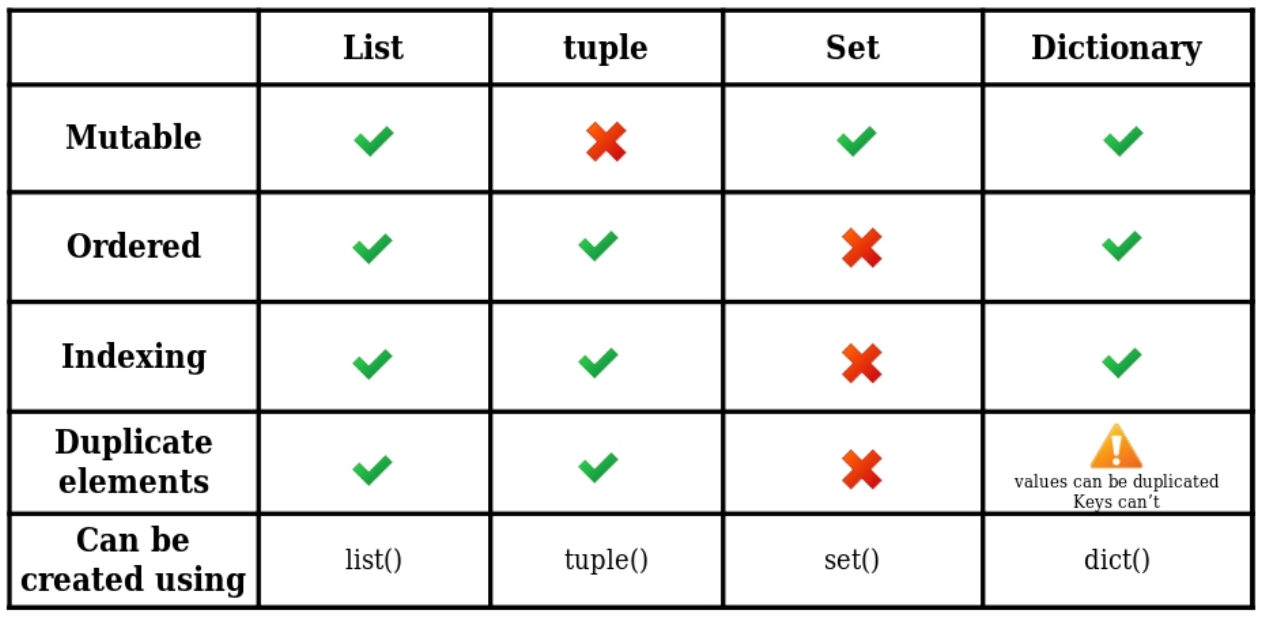
\includegraphics{/home/dbhenri/Documents/Cours python/PCBS/slides/intro-to-programming/2022/2nd class/python collections.png}
\end{frame}

\begin{frame}{Exercises 1}
\protect\hypertarget{exercises-1}{}
\begin{itemize}
\tightlist
\item
  Exercise 1: Lists: list1 = {[}1,2,3,4,1{]}

  \begin{itemize}
  \tightlist
  \item
    Given list1 print their sum with for and while loops
  \item
    Given list1 print their product for and while loops
  \item
    Given list1 print the sum of their squares for and while loops
  \item
    Given list1 print the largest number for and while loops
  \item
    Given list1 print the second largest for and while loops
  \end{itemize}
\item
  Exercise 2: Tuples

  \begin{itemize}
  \tightlist
  \item
    Given a list l={[}1, 2, 3, 6, 7, 4, 5{]}, transform it into a tuple
  \item
    Return the min and max of each tuples: truple = {[}(1,3,2), (6,4,5),
    (8,7,9){]}
  \item
    Given a list of tuples, return tuples that have all positive
    elements. test\_tuples = {[}(1,2,3), (4,5,6), (7,8,9), (-1,2,3){]}
  \end{itemize}
\item
  Exercise 3 : Sets

  \begin{itemize}
  \tightlist
  \item
    Order the tuples l from Exercise 2 and transform it into a Set
  \item
    Given a set Set1 = \{ 1,2,3,3,5,6,7\} remove the 4th items
  \item
    Given two sets a, b. Print True if they have items in common or
    False if not. a = \{``apple'', ``pineapple'', ``peach'', ``pears'',
    ``lemon'', ``lychee''\} b = \{``banana'', ``mango'' , ``lychee'',
    ``kiwi'', ``apple'', ``orange''\}
  \end{itemize}
\item
  Exercise 4: Given a list of words, count the number of times each word
  appears in the list (using dictionary)

  \begin{itemize}
  \tightlist
  \item
    animaList={[}``dog'', ``horse'', ``cat'', ``fish'', ``cat'',
    ``fox'', ``tiger'', ``tiger'', ``flamingo'', ``cat''{]}
  \end{itemize}
\end{itemize}
\end{frame}

\end{document}
